\documentclass{article}
\usepackage{geometry} \geometry{margin=1in}
\usepackage{parskip}
\usepackage{ragged2e}
\usepackage{float}       % Required for [H]
\usepackage{tcolorbox}
\usepackage{amsmath, amssymb}
\usepackage{tikz} 
\usetikzlibrary{shapes, arrows.meta, positioning, shadows}

% --- GLOBAL STYLE DEFINITIONS (The Chunk Prompt relies on these!) ---
\tikzset{
    block/.style={rectangle, draw, thick, rounded corners, fill=blue!5, align=center, minimum height=2em},
    arrow/.style={thick, ->, >=stealth},
    decision/.style={diamond, draw, fill=green!10, align=center, aspect=2}
}
\raggedbottom

\begin{document}

% --- START OF CHUNK 1 ---
\section{Fundamental Network Services and Ports}

In the study of cybersecurity, understanding the foundational communication protocols and their associated port numbers is crucial, as these ports represent the initial attack surface for many exploits. Network protocols define the rules for data exchange, while ports are logical endpoints used to differentiate between simultaneous services running on a single host. Monitoring, securing, and hardening these default ports are essential practices for network defense.

\begin{tcolorbox}[title=Common Network Protocols and Default Ports]
The following table summarizes key protocols frequently encountered in network environments:
\begin{center}
\begin{tabular}{|l|l|p{8cm}|}
\hline
\textbf{Protocol} & \textbf{Port(s)} & \textbf{Function/Relevance} \\
\hline
\textbf{FTP} & 20 (Data), 21 (Control) & \textbf{File Transfer Protocol}. Used for transferring files between a client and server. Due to its use of cleartext for credentials, it is often replaced by SFTP or FTPS. \\
\hline
\textbf{SSH} & 22 & \textbf{Secure Shell}. Provides secure, encrypted access for remote command execution and file transfer. A critical administrative tool. \\
\hline
\textbf{Telnet} & 23 & Used for interactive, text-oriented communication. Highly insecure as it transmits data in cleartext, making it obsolete for modern network management. \\
\hline
\textbf{SMTP} & 25 & \textbf{Simple Mail Transfer Protocol}. Used for sending email messages between servers. \\
\hline
\textbf{DNS} & 53 & \textbf{Domain Name System}. Translates domain names into IP addresses, a critical infrastructure service. \\
\hline
\textbf{HTTP} & 80 & \textbf{Hypertext Transfer Protocol}. The foundation of data communication for the World Wide Web, typically unsecured. \\
\hline
\textbf{POP3} & 110 & \textbf{Post Office Protocol version 3}. Used by local email clients to retrieve emails from a mail server. \\
\hline
\textbf{LDAP} & 389 & \textbf{Lightweight Directory Access Protocol}. Used to access and manage directory services information, such as user accounts and centralized policies. \\
\hline
\textbf{HTTPS} & 443 & \textbf{HTTP Secure}. Encrypted version of HTTP, utilizing TLS/SSL for secure communication over the web. \\
\hline
\textbf{RDP} & 3389 & \textbf{Remote Desktop Protocol}. Proprietary protocol developed by Microsoft, allowing users to remotely connect to another computer. High-value target for attackers seeking lateral movement. \\
\hline
\end{tabular}
\end{center}
\end{tcolorbox}

\section{The Evolving Classification of Security Professionals}

The term 'hacker' carries various connotations depending on the intent behind the access or manipulation of computer systems. In the field of cybersecurity, practitioners are generally categorized by the nature of their activities, often described using the metaphor of hat colors, distinguishing between ethical, malicious, and ambiguous behavior.

\subsection{White Hat Hackers}
A \textbf{white hat hacker} operates legally and ethically, serving as an asset to organizations by proactively identifying and remediating vulnerabilities. They are frequently referred to today as a \textbf{penetration tester} or Ethical Hacker. Their primary function is to simulate real-world attacks against a target system, but only with the explicit, written permission and authorization of the system owners. This sanctioned activity ensures that security flaws are found and fixed before malicious actors can exploit them.

\subsection{Black Hat Hackers (Crackers)}
In direct contrast, a \textbf{black hat hacker} gains unauthorized access to systems with the intention of causing harm, stealing data, disrupting services, or achieving financial gain through illegal means. Their actions are malicious and violate ethical and legal boundaries. Black hat hackers are sometimes referred to as \textbf{crackers}, a term that historically emphasized the breaking of security measures, particularly those related to intellectual property.

\subsection{Gray Hat Hackers}
A \textbf{gray hat hacker} occupies the middle ground. While they may generally be law-abiding citizens, they sometimes venture into activities that technically violate laws or ethical guidelines, often without inherently malicious intent. For example, a gray hat might discover a vulnerability in a company's system without permission, but then notify the company of the flaw. Although their ultimate goal may be public disclosure or security improvement, their initial unauthorized access classifies them distinctly from white hat professionals.

\section{Penetration Testing Methodology}

\subsection{Defining Penetration Testing}
\textbf{Penetration testing} is a controlled, authorized simulation of a cyber attack against a computer system, network, or application. Professionals who conduct these operations are known as \textbf{Ethical Hackers} or \textbf{Pen Testers}. The goal is to obtain authorization to simulate a full cyber attack against a target to identify security weaknesses. Pen Testers are typically employed by specialized security firms and provide a comprehensive report detailing any vulnerabilities found and concrete steps on how to fix the identified issues.

\subsection{Five High-Level Penetration Testing Stages}
The penetration test follows a structured methodology to ensure comprehensive coverage. One common framework divides the process into five distinct stages:

\begin{figure}[H]
    \centering
    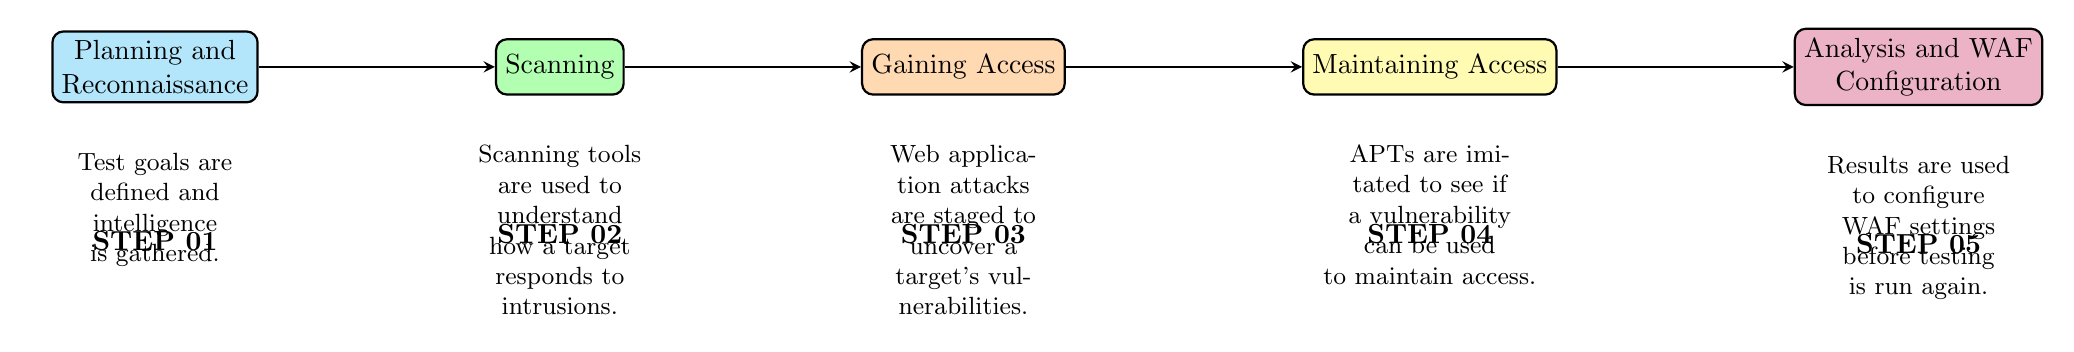
\begin{tikzpicture}[node distance=3cm, auto, thick]

    % Nodes
    \node[block, align=center, fill=cyan!30] (P1) {Planning and\\Reconnaissance};
    \node[block, right=of P1, align=center, fill=green!30] (P2) {Scanning};
    \node[block, right=of P2, align=center, fill=orange!30] (P3) {Gaining Access};
    \node[block, right=of P3, align=center, fill=yellow!30] (P4) {Maintaining Access};
    \node[block, right=of P4, align=center, fill=purple!30] (P5) {Analysis and WAF\\Configuration};

    % Descriptive Text (using standard text nodes for clarity)
    \node[text width=3cm, below=0.5cm of P1, align=center, font=\small] (D1) {Test goals are defined and\\intelligence is gathered.};
    \node[text width=3cm, below=0.5cm of P2, align=center, font=\small] (D2) {Scanning tools are used to\\understand how a target\\responds to intrusions.};
    \node[text width=3cm, below=0.5cm of P3, align=center, font=\small] (D3) {Web application attacks\\are staged to uncover a\\target's vulnerabilities.};
    \node[text width=3cm, below=0.5cm of P4, align=center, font=\small] (D4) {APTs are imitated to see if\\a vulnerability can be used\\to maintain access.};
    \node[text width=3cm, below=0.5cm of P5, align=center, font=\small] (D5) {Results are used to configure\\WAF settings before testing\\is run again.};

    % Arrows
    \draw[arrow] (P1) -- (P2);
    \draw[arrow] (P2) -- (P3);
    \draw[arrow] (P3) -- (P4);
    \draw[arrow] (P4) -- (P5);

    % Step Numbers
    \node[below=1.5cm of P1, font=\bfseries] {STEP 01};
    \node[below=1.5cm of P2, font=\bfseries] {STEP 02};
    \node[below=1.5cm of P3, font=\bfseries] {STEP 03};
    \node[below=1.5cm of P4, font=\bfseries] {STEP 04};
    \node[below=1.5cm of P5, font=\bfseries] {STEP 05};

    \end{tikzpicture}
    \caption{Five High-Level Stages of Penetration Testing}
\end{figure}

\subsection{Detailed Seven-Step Penetration Testing Flow}
A more granular representation of the penetration testing process highlights the iterative cycle of discovery, exploitation, and post-exploitation actions, particularly focusing on expanding scope and moving laterally within the target network.

\begin{figure}[H]
    \centering
    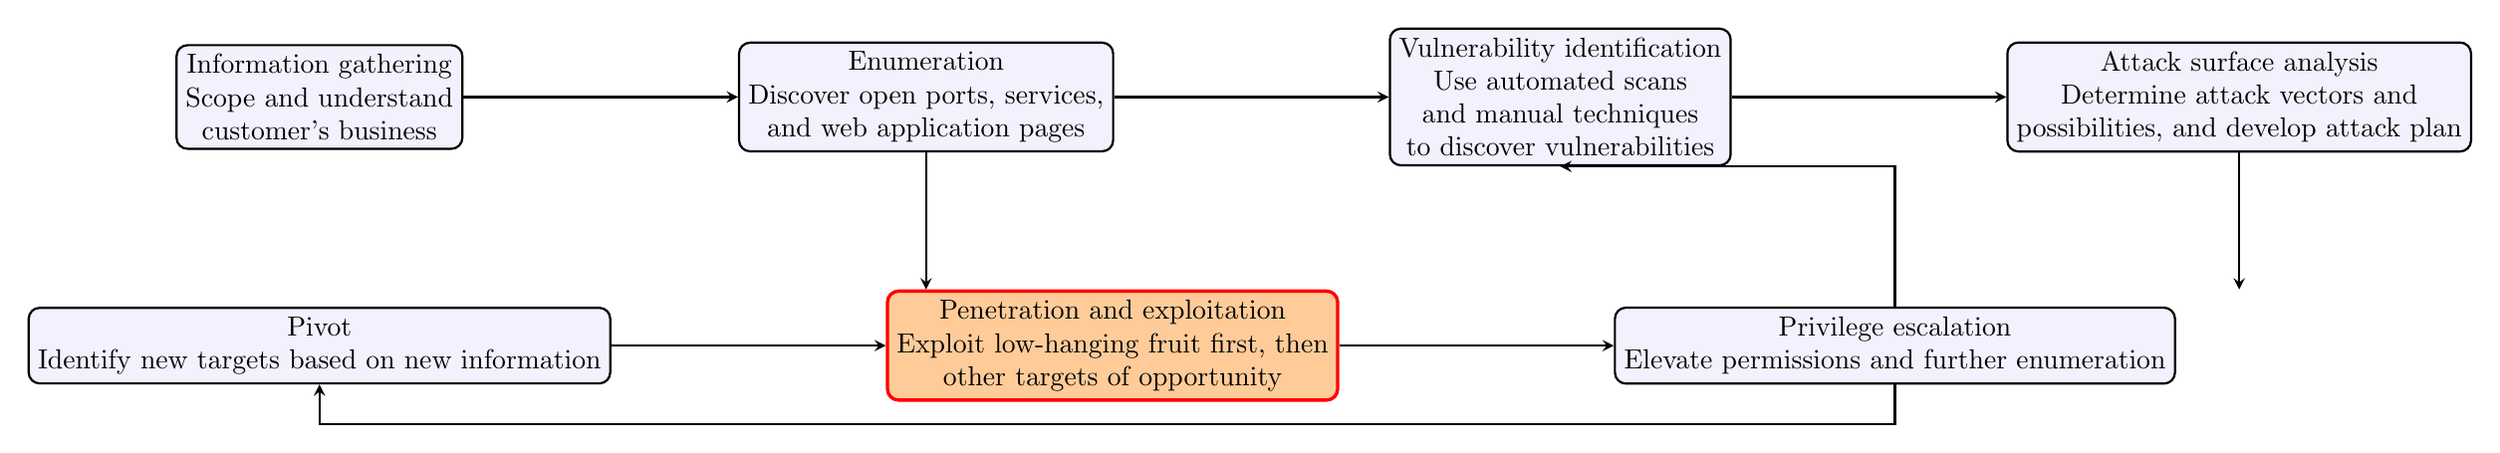
\begin{tikzpicture}[node distance=3.5cm and 3.5cm, auto, thick]

    % Row 1
    \node[block, align=center] (A) {Information gathering\\Scope and understand\\customer's business};
    \node[block, right=of A, align=center] (B) {Enumeration\\Discover open ports, services,\\and web application pages};
    \node[block, right=of B, align=center] (C) {Vulnerability identification\\Use automated scans\\and manual techniques\\to discover vulnerabilities};
    \node[block, right=of C, align=center] (D) {Attack surface analysis\\Determine attack vectors and\\possibilities, and develop attack plan};

    % Row 2
    \node[block, below=2cm of A, align=center] (E) {Pivot\\Identify new targets based on new information};
    \node[block, right=of E, align=center, fill=orange!40, draw=red, very thick] (F) {Penetration and exploitation\\Exploit low-hanging fruit first, then\\other targets of opportunity};
    \node[block, right=of F, align=center] (G) {Privilege escalation\\Elevate permissions and further enumeration};

    % Arrows (Horizontal Top)
    \draw[arrow] (A) -- (B);
    \draw[arrow] (B) -- (C);
    \draw[arrow] (C) -- (D);

    % Arrows (Connecting Rows)
    \draw[arrow] (D.south) -- (D.south |- F.north); % Attack plan leads down to exploitation
    \draw[arrow] (B.south) -- (B.south |- F.north); % Enumeration can also lead to exploitation
    \draw[arrow] (E.east) -- (F.west); % Pivot leads to exploitation

    % Arrows (Bottom Flow)
    \draw[arrow] (F) -- (G); % Exploitation leads to privilege escalation

    % Loops/Feedback
    % G to E (Privilege escalation leads to finding new targets/Pivot)
    \draw[arrow] (G.south) -- ++(0, -0.5) -| (E.south);
    % G to C (Privilege escalation leads to further vulnerability scanning/enumeration)
    \draw[arrow] (G.north) -- (G.north |- C.south) -- (C.south);

    \end{tikzpicture}
    \caption{Detailed Penetration Testing Flow Highlighting Iterative Steps}
\end{figure}

The steps in this detailed process cycle through intelligence gathering, discovery, and successful compromise:

\begin{enumerate}
    \item \textbf{Information Gathering}: Establishing the scope and thoroughly understanding the customer's business and network topography.
    \item \textbf{Enumeration}: Discovering exposed network services, open ports, and accessible web application pages.
    \item \textbf{Vulnerability Identification}: Employing both automated vulnerability scans and manual techniques to find exploitable weaknesses within the identified services.
    \item \textbf{Attack Surface Analysis}: Utilizing the collected vulnerability data to determine feasible attack vectors and developing a concrete plan of action for exploitation.
    \item \textbf{Penetration and Exploitation}: The critical phase where the tester actively exploits vulnerabilities, prioritizing easy targets (\textit{low-hanging fruit}) before attempting more complex exploits.
    \item \textbf{Privilege Escalation}: Post-exploitation actions focused on elevating permissions (e.g., from a standard user account to a root or system administrator account) to gain greater control, often followed by further enumeration.
    \item \textbf{Pivot}: Utilizing the compromised system as a launching point to identify and attack new targets laterally on the network that were previously shielded. This new information feeds back into the exploitation phase, restarting the discovery cycle on a new host.
\end{enumerate}

\section{The Open Web Application Security Project (OWASP)}

The \textbf{Open Web Application Security Project (OWASP)} is a globally recognized, non-profit foundation dedicated to improving the security of software. OWASP achieves its mission by focusing on practical security development and providing resources for developers and security professionals.

OWASP primarily provides three key resources:
\begin{itemize}
    \item \textbf{Tools}: Offering open-source projects and utilities designed to test and assess security.
    \item \textbf{Community and Networking}: Facilitating collaboration among security experts worldwide.
    \item \textbf{Education and Training}: Developing materials to increase security awareness and competency.
\end{itemize}

\subsection{The OWASP Top Ten List}
OWASP is renowned for publishing the \textbf{OWASP Top Ten}, a periodically updated report detailing the ten most critical security flaws found in software applications. This list serves as a vital benchmark for developers and organizations worldwide to prioritize security risks. The list is released approximately every three to four years, with the current iteration dating from 2021.

Vulnerabilities are assessed and ranked based on four main criteria:
\begin{itemize}
    \item \textbf{Exploitability}: How simple or complex the attack technique is.
    \item \textbf{Prevalence}: How frequently the vulnerability is discovered in web applications.
    \item \textbf{Detectability}: How easy it is for penetration testers or automated tools to find the flaw.
    \item \textbf{Technical Impact}: The potential severity of the harm caused if the vulnerability is successfully exploited.
\end{itemize}

\subsection{Evolution of the OWASP Top Ten (2017 to 2021)}
The transition from the 2017 list to the 2021 list involved significant reorganization, reflecting modern application architectures, the rise of API security concerns, and supply chain threats.

\begin{center}
\begin{tabular}{|c|l|c|l|}
\hline
\textbf{2017 Rank} & \textbf{2017 Flaw} & $\longrightarrow$ & \textbf{2021 Flaw (2021 Rank)} \\
\hline
A01 & Injection & $\longrightarrow$ & Injection (A03) \\
A02 & Broken Authentication & $\longrightarrow$ & Identification and Authentication Failures (A07) \\
A03 & Sensitive Data Exposure & $\longrightarrow$ & Cryptographic Failures (A02) \\
A04 & XML External Entities (XXE) & $\longrightarrow$ & Insecure Design (\textbf{A04 - New}) \\
A05 & Broken Access Control & $\longrightarrow$ & \textbf{Broken Access Control (A01)} \\
A06 & Security Misconfiguration & $\longrightarrow$ & Security Misconfiguration (A05) \\
A07 & Cross-Site Scripting (XSS) & $\longrightarrow$ & (Merged into A03 Injection) \\
A08 & Insecure Deserialization & $\longrightarrow$ & Software and Data Integrity Failures (\textbf{A08 - New}) \\
A09 & Using Components with Known Vulnerabilities & $\longrightarrow$ & Vulnerable and Outdated Components (A06) \\
A10 & Insufficient Logging \& Monitoring & $\longrightarrow$ & Security Logging and Monitoring Failures (\textbf{A09 - New}) \\
\hline
\multicolumn{4}{|c|}{\textbf{A10 (2021): Server-Side Request Forgery (SSRF)}} \\
\hline
\end{tabular}
\end{center}
The most notable change was the promotion of \textbf{Broken Access Control} to the number one spot, confirming that unauthorized access remains the most prevalent and impactful application flaw.

\subsection{A1: Broken Access Control}
Access control enforces security policy such that users are restricted to actions and resources authorized by their permissions. A \textbf{Broken Access Control} vulnerability arises when an application fails to properly enforce these restrictions, allowing users to manipulate parameters or circumvent checks to act outside of their intended boundaries.

Failures in access control can lead to devastating security consequences, as they allow an attacker to behave as a more privileged user. These failures typically result in:
\begin{itemize}
    \item Unauthorized disclosure of sensitive information.
    \item Modification or destruction of data, often system-wide.
    \item The ability to perform high-level business functions or administrative tasks that should be restricted.
\end{itemize}
Robust access control mandates validating every user request server-side, ensuring strict adherence to the principle of least privilege.

% --- START OF CHUNK 2 ---
\section{Access Control Vulnerabilities}
Access control, the process by which a system determines whether a user is authorized to perform a specific action, is a critical component of application security. Failures in this area often lead to serious security breaches, allowing unauthorized viewing, modification, or destruction of data.

The foundation of secure access control rests on the \textbf{principle of least privilege}, which dictates that a user or system process should only have the minimum permissions necessary to perform its function. Relatedly, the system should operate under a \textbf{deny by default} mechanism, where access is granted only when explicitly permitted. Violations of this principle constitute a major security flaw.

Common access control weaknesses include:
\begin{itemize}
    \item \textbf{Insecure Direct Object Reference (IDOR) and Parameter Tampering}: This occurs when an attacker modifies parameters within the URL (or other data fields) to bypass access controls. For example, changing a user ID from \texttt{user=123} to \texttt{user=456} to access someone else's account, potentially viewing or editing their data.
    \item \textbf{Vertical and Horizontal Privilege Escalation}: This involves an authorized user gaining access to resources they are not permitted to see. \textit{Horizontal escalation} involves accessing the data of a peer user (e.g., viewing another customer's account). \textit{Vertical escalation} involves a standard user gaining administrative rights or accessing pages meant only for privileged users (often referred to as \textbf{force browsing}).
    \item \textbf{Unauthenticated Access and Role Confusion}: This involves elevating privilege by acting as a user without being properly logged in, or accessing system functionality via APIs where authentication or authorization checks are completely missing, particularly for data modification methods like \textbf{POST}, \textbf{PUT}, and \textbf{DELETE}.
    \item \textbf{Metadata Manipulation}: This often involves tampering with or replaying session tokens or claims, such as a \textbf{JSON Web Token (JWT)}, to impersonate another user or modify the claims granting access rights.
\end{itemize}

\subsection{Web HTTP Methods and Status Codes}
To understand these vulnerabilities, it is necessary to grasp how web communications are handled using the underlying Hypertext Transfer Protocol (HTTP). The web sends data back and forth from the server to the client using specific HTTP Methods:
\begin{itemize}
    \item \textbf{GET}: Used to retrieve data or a resource from the server.
    \item \textbf{PUT}: Used to send updated data to the server, typically for replacing an existing resource.
    \item \textbf{POST}: Used to send new or created data to the server, often resulting in a new resource.
    \item \textbf{DELETE}: Used to remove data or a specific resource from the server.
\end{itemize}
Security implementations must ensure that modifying methods (\textbf{POST}, \textbf{PUT}, \textbf{DELETE}) are rigorously checked for authorization, as these methods can permanently alter application state.

When the server responds to a client request, it returns an \textbf{HTTP Status Code} to indicate the result of the request. These codes are grouped into five classes:

\begin{tcolorbox}[title=HTTP Status Code Classes]
\textbf{20X Success Codes}
\begin{itemize}
    \item 200 - OK: The request succeeded.
    \item 201 - Created: A new resource was created (common response to a POST request).
    \item 204 - No Content: The server successfully processed the request but is not returning any content (common response to a DELETE request).
\end{itemize}

\textbf{30X Redirection Codes}
\begin{itemize}
    \item 301 - Moved Permanently
    \item 304 - Not Modified
\end{itemize}

\textbf{40X Client Error Codes (Security Relevant)}
\begin{itemize}
    \item 400 - Bad Request: The server cannot process the request due to a client error.
    \item \textbf{401 - Unauthorized}: Authentication failed. The request requires user authentication credentials.
    \item \textbf{403 - Forbidden}: Authorization failed. The server understands the request but refuses to authorize access to the resource (e.g., a user is logged in, but lacks the necessary permissions).
    \item 404 - Not Found
\end{itemize}

\textbf{50X Server Error Codes}
\begin{itemize}
    \item 500 - Internal Server Error
    \item 503 - Service Unavailable
\end{itemize}
\end{tcolorbox}

\subsection{Mitigating Access Control Failures}
Preventing access control vulnerabilities requires strict adherence to security best practices throughout the development lifecycle:
\begin{enumerate}
    \item \textbf{Implement Deny by Default}: This is the foundational countermeasure. All access must be denied unless explicitly permitted by defined authorization rules.
    \item \textbf{Validate Authorization Context}: Before executing any action, especially those involving data modification (POST, PUT, DELETE), the application must verify two key facts: that the user is authenticated, and that the authenticated user is authorized to perform that specific action on that specific resource (ensuring the correct user is making the change and preventing IDOR).
    \item \textbf{Use Strong Identifiers}: To prevent simple parameter tampering attacks, identifiers (IDs) should be difficult to guess and non-sequential. Using universally unique identifiers (\textbf{GUIDs} or \textbf{UUIDs}) instead of simple numeric IDs makes enumeration attempts significantly harder.
    \item \textbf{Secure Authentication and Session Management}: Use tokens, such as \textbf{JWTs} (\texttt{https://jwt.io}), for robust authentication. These tokens must be properly signed and validated on the server side to prevent unauthorized tampering or replay attacks.
    \item \textbf{Enforce Secure Configuration}: Disable web server directory listing to prevent information leakage. Utilize \textbf{Cross-Origin Resource Sharing (CORS)} policies strictly to control which external domains can interact with the application’s resources.
    \item \textbf{Monitor and Audit}: Log all access control failures (401 and 403 responses) and review these logs periodically. Frequent failures may indicate active attack attempts or widespread security flaws requiring immediate remediation.
\end{enumerate}

\section{A2: Cryptographic Failures}
The current OWASP Top Ten list identifies \textbf{A2: Cryptographic Failures} (previously referred to as Sensitive Data Exposure) as a critical risk. This category addresses fundamental weaknesses in protecting sensitive data both when it is stored (\textbf{at rest}) and when it is transmitted (\textbf{in transit}).

Cryptographic failures can lead to the exposure of highly sensitive information, including:
\begin{itemize}
    \item Passwords and authentication credentials.
    \item Credit Card numbers and financial data.
    \item Health Records (subject to regulations like \textbf{HIPAA}).
    \item Personally Identifiable Information (\textbf{PII}), such as names, addresses, and social security numbers.
\end{itemize}

\subsection{Assessing Cryptographic Weakness}
A comprehensive security review must systematically evaluate the cryptographic hygiene of an application. Key questions to determine vulnerability include:
\begin{itemize}
    \item \textbf{Data Transmission Integrity}: Is any sensitive data transmitted across the network in \textbf{clear text}? All traffic, especially authentication and transactional data, must use secure protocols like HTTPS.
    \item \textbf{Algorithm Strength}: What version of cryptography is being used? Older, known-weak hashing algorithms, such as \textbf{SHA1} or \textbf{MD5}, should be banned and replaced with modern, salted, adaptive hashing methods (e.g., Argon2, bcrypt).
    \item \textbf{Key Management}: Are the default cryptographic keys used in the system weak, or are they being used across multiple servers? How were these keys generated, and are they protected according to industry best practices? Key leakage or weak key generation exponentially increases the risk of successful decryption by attackers.
    \item \textbf{Certificate Validation}: Is the certificate chain obtained from the Certificate Authority (\textbf{CA}) properly validated? Have any necessary security certificates expired, potentially forcing users to ignore warnings and establish insecure connections?
\end{itemize}

\subsection{Data Classification and Handling}
Effective cryptographic protection begins with data classification. It is essential to determine the sensitivity of all data elements being transmitted and stored to select the appropriate handling methods.

\subsubsection{Data Classification}
Data must be classified based on its inherent sensitivity and any applicable legal requirements:
\begin{itemize}
    \item \textbf{Confidentiality}: Is the data a company secret, financial record, or regulated PII?
    \item \textbf{Legal Requirements}: Does the data fall under regulatory frameworks such as HIPAA (Health Data) or GDPR/CCPA (PII)?
    \item \textbf{Authentication Credentials}: Is the data a password, PIN code, or security question answer, requiring specific, irreversible protection?
\end{itemize}

\subsubsection{Data Handling Based on Classification}
Once classified, the mechanism for storage and transmission must be chosen carefully:
\begin{itemize}
    \item \textbf{Passwords and PIN codes}: These must be protected using one-way transformation mechanisms. They should be \textbf{Hashed} using strong, salted algorithms, never encrypted, as they should never need to be converted back into clear text.
    \item \textbf{User Personal Information, Health Information, and Company Private Info}: Data that needs to be reversible (i.e., must be readable by the application later) must be strongly \textbf{Encrypted} both at rest and in transit.
    \item \textbf{Public Information (Company and User)}: Information intended to be publicly viewable can be stored and transmitted as \textbf{Plain Text}.
\end{itemize}

\subsubsection{Securing Data in Transit}
Using inherently secure protocols is vital for protecting data in transit:
\begin{itemize}
    \item \textbf{Web Traffic}: HTTP (Hypertext Transfer Protocol) is not secure. All websites that handle sensitive data must use \textbf{HTTPS} (HTTP Secure), which utilizes Transport Layer Security (TLS) encryption.
    \item \textbf{File Transfer}: FTP (File Transfer Protocol) is insecure. Servers must utilize \textbf{FTPS} (Secure File Transfer Protocol) or SFTP (SSH File Transfer Protocol) for secure file exchange.
    \item \textbf{Email (SMTP)}: The standard Simple Mail Transfer Protocol (SMTP) is not inherently secure. While there is no universally adopted, mandatory Secure Mail protocol, modern mail services (like Gmail) offer transport layer encryption or allow for the use of add-ons that facilitate end-to-end encryption.
\end{itemize}

\subsubsection{Secure Email Implementation}
Achieving true end-to-end secure email typically relies on \textbf{Public Key Cryptography}. Add-ons for email clients enable this functionality: the sender uses the recipient’s publicly available key to encrypt the message. Only the recipient possesses the corresponding private key necessary to decrypt and read the message. This method ensures confidentiality but requires coordination and key exchange between both the sender and receiver.

% --- START OF CHUNK 3 ---
\section{Secure Handling and Storage of Sensitive Data}

The storage and handling of consumer financial information are tightly regulated by the **Payment Card Industry Data Security Standard (PCI DSS)} set by the Payment Card Industry (PCI). These standards dictate the required security controls that organizations must implement to protect cardholder data.

The overarching principle of the PCI DSS is \textbf{data minimization}. Organizations are strongly discouraged from storing actual credit card numbers. If a web application requires payment information for recurring billing, the recommendation is to employ a strategy known as \textbf{tokenization}.

Tokenization involves replacing the sensitive Primary Account Number (PAN) with a non-sensitive, encrypted value (the token) generated by a credit card clearing company, such as First Data. This encrypted token can be stored locally, but since it is worthless outside the specific processing environment, it drastically reduces the organization's compliance scope and liability in the event of a breach.

\subsection{Principles of Data Minimization and Protection}

Beyond financial data, general principles apply to all sensitive personal information. The fundamental security recommendation is simple: \textbf{Do not store sensitive data if it is not absolutely necessary}.

If data storage is unavoidable, several techniques must be employed to mask or protect it:

\begin{itemize}
    \item \textbf{Truncation:} This involves retaining only a portion of the sensitive data, such as keeping only the last four digits of a Social Security Number (SSN) or credit card number, rendering the original data unusable by an attacker.
    \item \textbf{Encryption at Rest:} If the full data must be stored, it must be encrypted. Encryption transforms the data into an unreadable format, requiring a secure key for decryption.
    \item \textbf{Hashing for Comparison:} Data that only needs to be verified or compared (such as passwords) should be run through a one-way hashing algorithm. A hash is impossible to reverse-engineer to retrieve the original input, making it highly secure for comparison and matching purposes.
    \item \textbf{Data Isolation:} Where possible, the most sensitive data should be moved off the public-facing application server and isolated into a hardened, internal system.
\end{itemize}

\subsection{Cryptography and Regulatory Compliance}

Preventing data breaches requires proactive measures rooted in policy and technical implementation:

First, all data, whether processed, stored, or transmitted, must be subject to \textbf{data classification}. This involves categorizing the information into sensitivity levels (e.g., public, confidential, secret). This classification process must take into consideration various legal and regulatory requirements (e.g., HIPAA, GDPR) that dictate protection mandates.

Technically, systems must enforce robust cryptographic standards:
\begin{enumerate}
    \item All sensitive data must be \textbf{encrypted at rest} (when stored) using up-to-date and standard cryptography algorithms.
    \item All data transmission must utilize modern transport layer security, specifically using \textbf{TLS 1.2 or above}. Older protocols like SSL and earlier versions of TLS are considered deprecated and highly vulnerable.
    \item To prevent leakage of credentials or personal information, applications must be configured to \textbf{disable caching of sensitive data} on client-side browsers or intermediary systems.
\end{enumerate}

\section{A03: Understanding and Preventing Injection Attacks}

\textbf{Injection Attacks} are consistently listed among the most critical application security risks (often designated as A03 by the OWASP Top 10 list). These attacks occur when an application processes \textbf{untrusted data} without sufficient validation, allowing an attacker to inject hostile data that is then interpreted by the system as executable commands.

While the most famous and commonly exploited form is the \textbf{SQL Injection (SQLi)} attack, injection is a broad category encompassing several types of data execution vulnerabilities, including:
\begin{itemize}
    \item \textbf{NoSQL Injection} (targeting non-relational databases).
    \item \textbf{Command Injection} (allowing attackers to run operating system commands).
    \item \textbf{LDAP Injection} (targeting directory service queries).
\end{itemize}

\subsection{Indicators of Vulnerability}

An application is vulnerable to injection attacks if it exhibits any of the following traits:

\begin{itemize}
    \item \textbf{Lack of Validation:} User-supplied data is accepted and processed without stringent input validation, sanitization, or escaping.
    \item \textbf{Unparameterized Queries:} Dynamic database queries are built using simple string concatenation. The safest defense against SQLi is the use of \textbf{prepared statements} or parameterized queries, which ensure the database driver distinguishes between executable code (the query structure) and user input (the data).
    \item \textbf{Direct Usage of Hostile Data:} Hostile data is directly used or concatenated into the input stream, allowing the user's input to change the fundamental logic of the underlying command being executed.
\end{itemize}

\section{Relational Database Fundamentals}

One of the most efficient and structured ways to store and manage data is through a \textbf{relational database}. Relational databases organize data to reveal relationships between different data points, ensuring integrity and consistency.

Relational data is structured into named entities called \textbf{Tables}. Tables are composed of \textbf{Columns} (which define the data attributes or fields, such as "Name" or "Email") and \textbf{Rows} (which represent individual records or instances of data). For example, in a "Users" table, the columns would define attributes like ID, Name, Username, and Password, while each row would contain the specific data for a single user.

These structured tables can be queried, manipulated, and managed using a highly standardized and robust language known as \textbf{Structured Query Language (SQL)}.

\subsection{Common Database Management Systems (DBMS)}

Relational databases are managed by Database Management Systems (DBMS), which are broadly categorized by licensing and use case:

\begin{itemize}
    \item \textbf{Free/Open Source Options:} Popular open-source systems include \textbf{MySQL} and \textbf{PostgreSQL}. MySQL, which is owned by Oracle, remains one of the most widely deployed free relational databases due to its performance, reliability, and support for multiple operating systems, including Windows, MacOS, and Unix-based platforms.
    \item \textbf{Enterprise Options:} These commercial systems are often deployed in large-scale corporate environments and include Microsoft SQL Server, Oracle, and IBM DB2.
\end{itemize}

\subsection{Data Manipulation: CRUD Operations}

All relational database systems must provide a means to manage persistent data through four essential functions, collectively known as \textbf{CRUD}: Create, Read, Update, and Delete. These abstract operations map directly to specific keywords in SQL used to interact with the stored data.

\begin{tcolorbox}[title=SQL CRUD Operations]
\begin{itemize}
    \item \textbf{Create:} Used to add new rows of data to a table, corresponding to the SQL command \texttt{INSERT INTO}.
    \item \textbf{Read:} Used to retrieve existing data from the database, corresponding to the SQL command \texttt{SELECT}.
    \item \textbf{Update:} Used to modify existing data in one or more rows, corresponding to the SQL command \texttt{UPDATE}.
    \item \textbf{Delete:} Used to remove one or more rows of data from a table, corresponding to the SQL command \texttt{DELETE}.
\end{itemize}
\end{tcolorbox}

% --- START OF CHUNK 4 ---
\section{The Fundamentals of SQL Data Manipulation Language (DML)}

Structured Query Language (\textbf{SQL}) is the standard language for managing and querying data stored in relational database management systems (RDBMS). Data Manipulation Language (DML) encompasses the core operations required to handle data records within a table: Read, Create, Update, and Delete (CRUD). Understanding the precise syntax and structure of these operations is foundational to both database management and security analysis.

\subsection{Reading Data: The \texttt{SELECT} Statement}

The most frequently used SQL operation is the \texttt{SELECT} statement, used for retrieving data records from one or more tables. The basic structure requires specifying which columns are desired and from which table the data should be drawn:

\[
\texttt{SELECT [columns] FROM [table]}
\]

The \texttt{[columns]} argument specifies the attributes to be returned. This can be a single column, or multiple column names provided in a comma-delimited list. Alternatively, the asterisk symbol (\texttt{*}) is used as a wildcard to signify that all columns from the specified table should be returned.

\begin{tcolorbox}[title=Examples of SELECT Queries]
\begin{enumerate}
    \item Retrieving all data from the \texttt{Users} table:\\
    \texttt{SELECT * FROM Users}
    \item Retrieving only the names and emails:\\
    \texttt{SELECT Name, Email FROM Users}
\end{enumerate}
\end{tcolorbox}

\subsection{Filtering Data: The \texttt{WHERE} Clause}

While the basic \texttt{SELECT} retrieves all rows, filtering records based on specific criteria is essential. This is achieved using the \textbf{\texttt{WHERE}} clause. The \texttt{WHERE} clause restricts the rows returned by applying conditional logic.

The general structure of a filtered query is:
\[
\texttt{SELECT [columns] FROM [table] WHERE [column] = [value]}
\]

The condition specified after \texttt{WHERE} dictates which rows are included in the final result set.

\begin{tcolorbox}[title=Condition Filtering Examples]
\begin{enumerate}
    \item Retrieving the record where the Name is exactly 'Jeff':\\
    \texttt{SELECT * FROM Users WHERE Name='Jeff'}
    \item Retrieving the record where the numeric identifier (\texttt{Id}) is 2:\\
    \texttt{SELECT * FROM Users WHERE Id=2}
\end{enumerate}
\end{tcolorbox}

\subsubsection{Advanced Filtering with \texttt{LIKE}}

For pattern matching rather than exact equality, the \textbf{\texttt{LIKE}} operator is employed, often in conjunction with the percent symbol (\texttt{\%}) wildcard. The wildcard represents zero or more characters.

For instance, to retrieve all users whose names begin with the letter 'J':
\[
\texttt{SELECT * FROM Users WHERE Name LIKE 'J\%'}
\]

\subsection{Creating Data: The \texttt{INSERT INTO} Statement}

The \texttt{INSERT INTO} statement is used to add new records (rows) into an existing table. When creating data, it is crucial that the number of columns specified matches the number of values provided, and that the data types align.

The required syntax structure is:
\[
\texttt{INSERT INTO [table] ([columns]) VALUES ([values])}
\]

\begin{tcolorbox}[title=Example of INSERT INTO]
To add a new user named Hank with Id 4:
\[
\texttt{INSERT INTO Users (Id, Name, Email,...) VALUES (4, 'Hank', 'hank@okcu.edu',...)}
\]
\end{tcolorbox}

\subsection{Modifying Data: The \texttt{UPDATE} Statement}

The \texttt{UPDATE} statement is used to modify existing records in a table. It requires specifying the table, using the \texttt{SET} keyword to define the new values for specific columns, and, critically, using the \texttt{WHERE} clause to specify which rows should be affected.

\[
\texttt{UPDATE [table] SET [column]=[value] WHERE [column]=[value]}
\]

\textbf{Caution:} It is imperative to include a \texttt{WHERE} clause when using \texttt{UPDATE}. If the \texttt{WHERE} clause is omitted, the specified changes will be applied to \emph{every single record} in the table, potentially leading to widespread data corruption.

\begin{tcolorbox}[title=Example of UPDATE]
To change the name of the user with Id 1 to 'Jeff Maxwell':
\[
\texttt{UPDATE Users SET Name='Jeff Maxwell' WHERE Id=1}
\]
\end{tcolorbox}

\subsection{Removing Data: The \texttt{DELETE} Statement}

The \texttt{DELETE FROM} statement permanently removes rows from a table. Like \texttt{UPDATE}, it relies entirely on the \texttt{WHERE} clause to target specific records for deletion.

\[
\texttt{DELETE FROM [table] WHERE [column]=[value]}
\]

\textbf{Extreme Caution:} Omitting the \texttt{WHERE} clause in a \texttt{DELETE FROM} statement will result in the deletion of \emph{all records} in the table. This operation is often irreversible without recent backups.

\begin{tcolorbox}[title=Example of DELETE]
To delete the user record with Id 1:
\[
\texttt{DELETE FROM Users WHERE Id=1}
\]
\end{tcolorbox}

\section{Introduction to SQL Injection}

SQL Injection is one of the most common and dangerous web application vulnerabilities. It occurs when an attacker can interfere with the queries that an application makes to its database, allowing them to view, modify, or delete data they are not authorized to access.

\subsection{The Context: A Sample User Table}

To illustrate the vulnerability, we use a hypothetical \texttt{Users} table, representative of an authentication database schema:

\begin{figure}[H]
    \centering
    \caption{Hypothetical \texttt{Users} Table Data}
    \begin{tabular}{|l|l|l|l|l|}
        \hline
        \textbf{Id} & \textbf{Name} & \textbf{Username} & \textbf{Email} & \textbf{Password} \\
        \hline
        1 & Jeff & Jmaxwell & jmaxwell@okcu.edu & Password\#123 \\
        \hline
        2 & John & Jsmith & jsmith@okcu.edu & Password\#123 \\
        \hline
        3 & Jane & jsmith2 & jsmith2@okcu.edu & Password\#123 \\
        \hline
    \end{tabular}
\end{figure}

A standard login screen checks the provided username and password against a query to this database. If a matching row is found, the user is authenticated.

\subsection{How SQL Injection Works}

The vulnerability arises primarily from the practice of constructing SQL queries using simple string concatenation based on user input, rather than using parameterized queries.

\subsubsection{The Expected Query Construction}
If a user attempts to log in with username \texttt{jmaxwell} and password \texttt{Password\#123}, the application code (often written in a language like Java or PHP) dynamically builds the following query string:

\begin{verbatim}
SELECT * FROM Users WHERE username='jmaxwell' AND password='Password#123';
\end{verbatim}

The application code often handles this concatenation similarly to:
\begin{verbatim}
String sql = "SELECT * FROM Users WHERE username='" + username
           + "' AND password='" + password + "'";
\end{verbatim}

\subsubsection{Exploitation via Logical Bypass}

An attacker exploits this vulnerability by entering malicious characters into the input fields, specifically characters that change the logical structure of the resulting SQL query.

Consider an attacker who enters the username \texttt{jmaxwell} and uses a malicious input for the password field: \texttt{jmaxwell' or '1'='1' --}.

When the application concatenates this input, the resulting SQL query becomes drastically altered:
\begin{verbatim}
SELECT * FROM Users WHERE username='jmaxwell'
    OR '1'='1' -- AND password='xxx'
\end{verbatim}
(Note: We use \texttt{xxx} here to represent whatever else the application expected to wrap the password input.)

\paragraph{Analysis of the Malicious Query:}
\begin{enumerate}
    \item The attacker's first single quote (\texttt{'}) closes the quote initiated by the application for the username parameter.
    \item The \texttt{OR '1'='1'} segment is injected. Since the condition $1=1$ is always true, the entire \texttt{WHERE} clause now evaluates to true for the first record encountered.
    \item The double hyphen (\texttt{--}) is a standard SQL comment operator. This operator effectively causes the database engine to ignore the rest of the original query, including the subsequent \texttt{AND password='xxx'} section.
\end{enumerate}

Because the \texttt{WHERE} clause evaluates to true for the first user record (Id 1, Jeff), the database returns that row. If the application logic simply checks if \emph{any} rows were returned, the attacker is successfully authenticated as Jeff, regardless of the correct password. This ability to inject logical conditions (\texttt{OR 1=1}) and terminate the remainder of the query (\texttt{--}) demonstrates the core mechanism of a classic SQL injection attack.

% --- START OF CHUNK 5 ---
\section{A04: Insecure Design and Secure Design Principles}

\subsection{The OWASP Top 10: Insecure Design (A04)}

\textbf{Insecure Design} (A04) was introduced to the OWASP Top 10 in 2021, marking a shift toward recognizing architectural and design deficiencies as a major source of application risk. This category is exceptionally broad, encompassing issues that arise not from faulty coding practices, but from fundamental security flaws embedded in the system's architecture.

The most critical symptom of Insecure Design is the \textbf{Missing or Ineffective Control Design}. This means that security controls were either entirely overlooked during the planning phase or were designed inadequately to meet modern threat vectors. When evaluating a system architecture, academic focus must therefore shift to critical questions regarding risk:
\begin{itemize}
    \item What specific \textbf{risks} are introduced by this design? This includes risks related to trust boundaries, unauthorized data access, or the inability to enforce separation of duties.
    \item How are these identified risks currently being \textbf{managed} and mitigated? A robust design must clearly articulate the control mechanisms used to reduce the probability or impact of identified threats.
\end{itemize}

\subsection{Defining Secure Design}

Secure Design is far more than a technical blueprint or a simple diagram; it is a foundational change in organizational philosophy. It mandates a transformation in thinking, culture, and approach concerning the development of both software and hardware systems.

\begin{tcolorbox}[title=Definition]
\textbf{Secure Design} requires integrating security considerations, defined methodologies, and architectural patterns from the very initial phase of system conceptualization. Its goal is to ensure that security is a non-negotiable, inherent quality of the system, not an add-on or a post-development fix.
\end{tcolorbox}

Organizations must adopt structured methodologies (such as security requirements engineering and dedicated architecture review) and maintain a constant, corporate-wide drive to prioritize security improvements, starting precisely with the system design.

\section{Risk Management through Threat Modeling}

\subsection{Introduction to Threat Modeling}

\textbf{Threat Modeling} is the proactive, structured practice of reviewing current application diagrams, data flow maps, and architectural specifications to identify potential security issues inherent in the design itself. By examining the system from an attacker's perspective, architects can anticipate how assets might be compromised.

Effective threat modeling focuses on critical interrogation points within the system design to ensure adequate controls are in place:
\begin{itemize}
    \item \textbf{Data Flow Analysis:} Defining how information moves between trust boundaries and components.
    \item \textbf{Encryption Verification:} Checking if appropriate cryptographic measures are being used for data in transit and at rest.
    \item \textbf{Access Control Mapping:} Clearly establishing \textbf{who} (users, roles, services) has access to \textbf{what} specific data or functionality.
\end{itemize}

\subsection{Example: Application Architecture Diagram}
The following diagram illustrates a multi-tiered application architecture used for threat analysis. Key elements requiring security scrutiny include the demarcation of trust zones (DMZ, LAN, Restricted Network) and the placement of authentication and encryption controls.

\begin{figure}[H]
\centering
\begin{tikzpicture}[node distance=1.5cm, auto]

% Define nodes based on the diagram flow
\node[block] (users) {Users};
\node[block] (webserver) [right=2cm of users] {Web Server};
\node[block] (appserver) [below right=1.5cm of webserver] {Application Server};
\node[block] (dbserver) [below right=1.5cm of appserver] {Database Server};
\node[block] (finserver) [right=3cm of webserver, yshift=-0.5cm] {Financial Server};

% Trust Zones
\node[draw, dashed, inner sep=1cm, fit=(users) (webserver)] (dmz) {};
\node[block, below left=0.1cm of dmz.south west, align=left] {DMZ};

\node[draw, dashed, inner sep=1cm, fit=(appserver) (dbserver)] (lan) {};
\node[block, below left=0.1cm of lan.south west, align=left] {LAN};

\node[draw, dashed, inner sep=1cm, fit=(finserver)] (restricted) {};
\node[block, below right=0.1cm of restricted.south east, align=right] {Restricted Network};


% Draw connections and labels
\draw[arrow] (users) -- (webserver) node[midway, above] {Request};
\draw[arrow] (webserver) -- (users) node[midway, below] {Responses};

% Web Server to App Server
\draw[arrow] (webserver) to[bend right] (appserver) node[midway, above left] {Application Calls};
\draw[arrow] (appserver) to[bend right] (webserver) node[midway, below right] {Message Response};

% App Server to DB Server
\draw[arrow] (appserver) -- (dbserver);
\node[block, right=0.5cm of webserver.east, yshift=0.5cm] (message) {Message};
\draw[arrow] (webserver) -- (message);
\draw[arrow] (message) -- (finserver);

% DB controls
\node[block, align=center] (dbenc) [below=0.5cm of dbserver] {Encryption\\+ Authentication};
\draw[arrow] (dbenc) -- (dbserver);

% App Server controls
\node[block, align=center] (appenc) [left=0.5cm of appserver.south west] {Encryption\\+ Authentication};
\draw[arrow] (appenc) -- (appserver);


\node[block] (authd) [below left=1cm of dbserver] {Auth Data};
\draw[arrow] (dbserver) -- (authd);
\node[block] (sql) [below right=1cm of dbserver] {SQL Query};
\draw[arrow] (dbserver) -- (sql);

\node[block] (authdata) [below=1cm of sql] {Authentication Data};
\draw[arrow] (sql) -- (authdata);

% Financial Server flow
\node[block] (custdata) [below=1.5cm of finserver] {Customer\\Financial Data};
\draw[arrow] (finserver) -- (custdata);

\node[block] (findata) [below=2.5cm of finserver] {Financial Data};
\draw[arrow] (custdata) -- (findata);

\node[block, align=center] (acctcalls) [right=1.5cm of finserver, yshift=1cm] {Account/Transaction\\Query Calls};
\draw[arrow] (finserver) -- (acctcalls);

% Restricted Network boundary
\draw[dashed, fit=(finserver) (custdata) (findata) (acctcalls)] (restricted);
\draw[arrow] (sql) -- (restricted.south west);

\end{tikzpicture}
\caption{Threat Modeling Data Flow Diagram Example}
\end{figure}

\subsection{Example: Banking Transaction Data Flow}
Analyzing business process flows, such as a banking withdrawal, allows for the identification of potential gaps in authorization enforcement. The following diagram focuses on the decision points for authentication (AuthN) and authorization (AuthZ) and highlights how sensitive information (like bad account lists or policy checks) interacts with the core transaction process.

\begin{figure}[H]
\centering
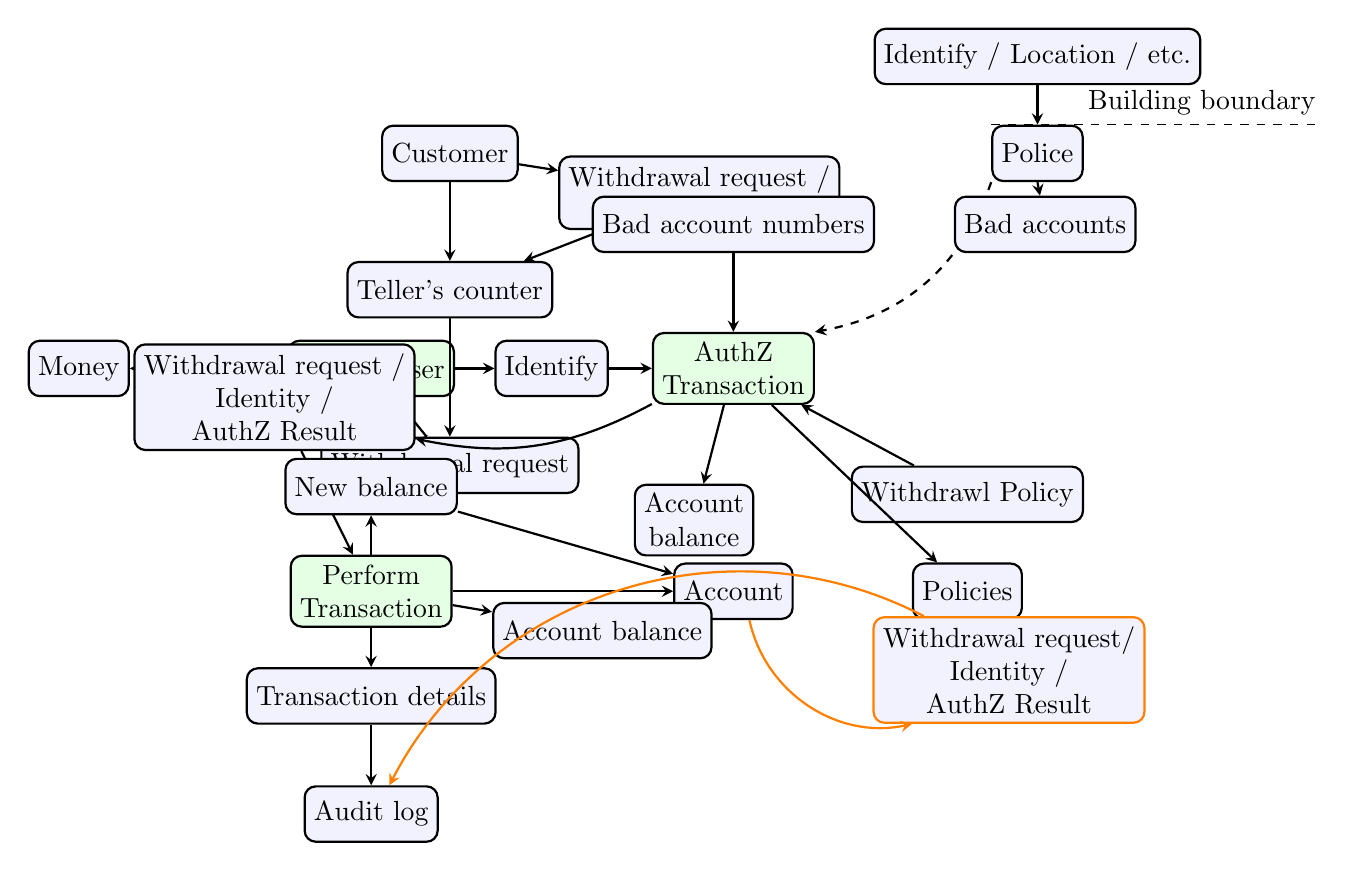
\begin{tikzpicture}[node distance=2cm, auto]

% Define Actors (Red/Rectangle)
\node[block] (customer) {Customer};
\node[block] (police) [right=6cm of customer] {Police};

% Define Processes (Green/Circle)
\node[block, draw, rounded corners, fill=green!10] (authn) [below=2cm of customer, xshift=-1cm] {AuthN User};
\node[block, draw, rounded corners, fill=green!10] (authz) [right=2.5cm of authn] {AuthZ\\Transaction};
\node[block, draw, rounded corners, fill=green!10, align=center] (perform) [below=2cm of authn] {Perform\\Transaction};

% Define Data/Entities (White/Block)
\node[block] (teller) [below=1cm of customer] {Teller's counter};
\node[block] (account) [below=2cm of authz] {Account};
\node[block] (policies) [right=1.5cm of account] {Policies};
\node[block] (audit) [below=2cm of perform] {Audit log};

% Flow from Customer/Teller
\node[block, align=center] (req1) [right=0.5cm of customer.east, yshift=-0.5cm] {Withdrawal request /\\ Identification};
\draw[arrow] (customer) -- (teller);
\draw[arrow] (customer) -- (req1);
\draw[arrow] (req1) -- (teller);

\node[block] (money) [left=2cm of authn] {Money};
\draw[arrow] (authn) -- (money);

% Teller to AuthN/AuthZ
\node[block] (req2) [below=0.5cm of authn, xshift=1cm] {Withdrawal request};
\draw[arrow] (teller) -- (req2);
\draw[arrow] (req2) -- (authn);

\node[block] (identify) [right=0.5cm of authn] {Identify};
\draw[arrow] (authn) -- (identify);
\draw[arrow] (identify) -- (authz);

% AuthZ controls and boundaries
\node[block, align=center] (accbal) [below=1cm of authz, xshift=-0.5cm] {Account\\balance};
\draw[arrow] (authz) -- (accbal);

\node[block] (wpolicy) [above=0.5cm of policies] {Withdrawl Policy};
\draw[arrow] (wpolicy) -- (authz);
\draw[arrow] (authz) -- (policies);

\node[block] (badnums) [above=1cm of authz] {Bad account numbers};
\draw[arrow] (badnums) -- (authz);

% Police/Building Boundary
\node[block] (loc) [above=0.5cm of police] {Identify / Location / etc.};
\draw[arrow] (loc) -- (police);
\draw[dashed, arrow] (police.south west) to[bend left] (authz.north east);
\node[block] (badaccounts) [right=1cm of badnums] {Bad accounts};
\draw[arrow] (police.south) -- (badaccounts);
\draw[dashed] (police.north west) -- (police.north east) -- node[midway, above] {Building boundary} ++(3, 0);

% AuthZ to Perform Transaction (AuthZ Result)
\node[block, align=center] (authzreq) [left=0.5cm of authn.south east] {Withdrawal request /\\ Identity /\\ AuthZ Result};
\draw[arrow] (authz) to[bend left=20] (authzreq);
\draw[arrow] (authzreq) -- (perform);

% Perform Transaction flows
\node[block] (newbal) [above=0.5cm of perform] {New balance};
\draw[arrow] (perform) -- (newbal);
\draw[arrow] (newbal) -- (account);
\draw[arrow] (perform) -- (account);

\node[block] (acctdet) [below=0.5cm of perform] {Transaction details};
\draw[arrow] (perform) -- (acctdet);

\node[block] (acctbal) [right=0.5cm of perform, yshift=-0.5cm] {Account balance};
\draw[arrow] (perform) -- (acctbal);

% Return loop (Orange path)
\node[block, align=center, draw=orange] (returnval) [right=1cm of account, yshift=-1cm] {Withdrawal request/\\ Identity /\\ AuthZ Result};
\draw[arrow, orange] (account) to[bend right=45] (returnval);
\draw[arrow, orange] (returnval) to[bend right=45] (audit);
\draw[arrow] (acctdet) -- (audit);

\end{tikzpicture}
\caption{Threat Modeling Example: Banking Withdrawal Data Flow Diagram}
\end{figure}

\section{Data Governance and Flow Analysis}

Robust Secure Design necessitates detailed governance over the data itself and strict control over its movement throughout the system architecture.

\subsection{Data Management Concerns}
Before deployment, system designers must finalize data classification, storage parameters, and access policies:
\begin{itemize}
    \item \textbf{Data Inventory:} What categories of data are being stored? This inventory must guide the subsequent application of security controls.
    \item \textbf{Classification Standards:} How is the data classified (e.g., Public, Confidential, Highly Sensitive)? Classification dictates the mandatory security measures (e.g., access logging, encryption standards).
    \item \textbf{Cryptographic Justification:} What data is being \textbf{Hashed/Encrypted}? A clear operational reason must be established for cryptographic protection, and, equally important, a justification (\textbf{Why Not?}) must exist for any sensitive data transmitted or stored in the clear.
    \item \textbf{Access Matrix:} Defining an explicit matrix showing \textbf{who} (which user role, application service, or external system) has verified, permissible access to the data.
    \item \textbf{External Sharing:} What data is being sent to other sources, such as external companies, APIs, or third-party processors? This data flow introduces external trust boundaries that require contractual and technical security assurances.
\end{itemize}

\subsection{Analyzing Data Flow}

Data flow analysis focuses on the movement and transformation of information between components, ensuring that security boundaries are respected during transfer. Key considerations include:
\begin{itemize}
    \item \textbf{Inter-System Flow:} How does the data flow between interconnected systems and services? Every transfer point is a potential exposure risk.
    \item \textbf{Inputs/Outputs Integrity:} What data enters and exits the system, and are the inputs and outputs validated and filtered against expected formats to prevent injection or corruption?
    \item \textbf{Transport Security:} Is the data transferred in \textbf{plain text} or \textbf{cipher text}? All data crossing trust boundaries, especially network boundaries, should use strong transport security.
    \item \textbf{Encryption Methods:} If cipher text is utilized, what specific encryption methods are being used (e.g., TLS version, cipher suites, key management practices), and are they compliant with current best practices?
\end{itemize}

\section{Security Assessment and Prevention}

\subsection{Performing Security Assessments}

Secure Design must be validated through formal assessments that check the theoretical design against the implemented reality. Continuous assessment is vital for maintaining security posture:
\begin{itemize}
    \item \textbf{Assessment Status:} Has a security assessment, such as a penetration test or architectural review, been formally performed on the application or system?
    \item \textbf{Assessment Recency:} When was the last assessment conducted? Designs evolve, and regular reassessment is crucial.
    \item \textbf{Findings and Remediation:} What were the key findings of the assessment? Tracking remediation of design flaws found during these tests is paramount.
    \item \textbf{Methodology:} How was the assessment performed? Did it utilize standardized, reproducible methodologies?
\end{itemize}

Organizations can measure and improve their overall capacity for secure software practices using the \textbf{OWASP Software Assurance Maturity Model (SAMM)}. SAMM provides a flexible framework to help organizations formulate and implement a strategy tailored to their specific risks and resources. Details can be found at \url{https://owaspsamm.org}.

\subsection{Preventing Insecure Design}

Preventing insecure design requires institutionalizing security within the development lifecycle through specific roles, tooling, and documentation requirements:
\begin{enumerate}
    \item \textbf{Early AppSec Integration:} Application Security (AppSec) professionals must be mandatory participants in the design phase. They should initiate discussions about security requirements and threat landscapes early in the design progress.
    \item \textbf{Secure Design Library:} Organizations should build and curate a library of established \textbf{Secure Design patterns} and reference examples of secure code. This minimizes the risk of individual teams inventing insecure solutions for common problems.
    \item \textbf{Systemic Threat Modeling:} Use Threat Modeling not only for general awareness but specifically for critical systems. This includes diagramming and enforcing all aspects of the authentication, access control, and authorization patterns utilized.
    \item \textbf{Data Flow Documentation:} Thoroughly diagramming and documenting the entire data flow between all systems is essential. This documentation serves as the foundational artifact for all subsequent risk analysis, security audits, and compliance checks.
\end{enumerate}

% --- START OF CHUNK 6 ---
\section{Application Security Validation and Defense}

To ensure application resilience against common threats—such as \textbf{SQL Injection}, \textbf{Cross-Site Scripting (XSS)}, and \textbf{Cross-Site Request Forgery (CSRF)}—development teams must formalize security testing early in the development lifecycle. This involves creating detailed user stories and functional requirements specifically designed to test and validate that the system cannot be exploited by known attack vectors. Furthermore, thorough testing of the system design itself is crucial to uncover architectural flaws before deployment. Finally, external validation through a professional \textbf{Penetration Tester} (PenTester) is essential, allowing an independent security expert to actively attempt to compromise the application and servers within the system to discover real-world weaknesses.

\section{A05: Security Misconfiguration}

The fifth item on the OWASP Top 10 list addresses \textbf{Security Misconfiguration (A05)}. This category encompasses flaws arising when systems, applications, or software components are not set up or maintained correctly according to secure operational standards. Misconfiguration is one of the most common vulnerabilities because it is easy to overlook simple settings that can have profound security implications. Attackers frequently seek out unpatched flaws—vulnerabilities that have already been publicly disclosed but remain unfixed. They also target organizational shortcomings, such as unprotected, accessible files and folders, and frequently exploit default configurations, which often leave servers unnecessarily exposed and vulnerable to exploitation.

\subsection{Manifestations of Security Misconfiguration}

Security misconfigurations manifest in numerous ways across the system architecture:
\begin{itemize}
    \item \textbf{Lack of OS/System Hardening}: Failure to apply necessary configuration controls to reduce the attack surface of the operating system or server software.
    \item \textbf{Missing Patches}: Operating systems and applications are missing the latest security updates or patches, often leaving holes open that are simple to exploit.
    \item \textbf{Excessive Services/Features}: Services or features are running that are unnecessary for the application's function and should have been removed or disabled.
    \item \textbf{Open Ports or Protocols}: Network ports are left open or non-essential network protocols are enabled, creating unnecessary exposure points.
    \item \textbf{Insecure Error Handling}: Error messages expose sensitive data, such as showing a full stack trace, which provides attackers with valuable internal security information about the system structure and technology versions.
    \item \textbf{Excessive Default Access}: Relying on default settings which frequently grant too much access or privilege to users or services, violating the principle of least privilege.
\end{itemize}

\subsection{Root Causes of Misconfiguration}

This pervasive vulnerability arises due to a combination of human error and process failure. Frequently, system administrators deploy and configure systems without full knowledge of the secure default values or the optimal secure state of the software. Without rigorous training or standardized deployment scripts, secure settings are often skipped. Furthermore, organizations often fail to implement robust, automated tools for patch management, leading to critical systems being overlooked or missing required security updates. A common and dangerous pitfall is the reliance on the insecure default configurations provided by vendors, rather than implementing a customized, hardened baseline before deployment.

\subsection{Preventing Security Misconfiguration}

Preventing security misconfiguration requires a rigorous and proactive approach to system administration and deployment:

\begin{enumerate}
    \item \textbf{System Hardening}: Collaborate closely with network and system administrators to "harden" the server, a process often described as "locking it down." This process must include removing any default accounts (or immediately changing their default credentials), disabling all unused services, and turning off any unused network ports.
    \item \textbf{Least Privilege}: Implement the principle of \textbf{least privilege} across the entire system. This critical security policy ensures that every user, process, and application component has only the minimum permissions necessary to perform its required task.
    \item \textbf{Standardized Secure Builds}: Create a secure, hardened baseline version of each operating system image or server template that can be used when building new systems. This prevents new systems from inheriting insecure default configurations.
    \item \textbf{Secure Error Handling}: Implement default error handling routines that prevent sensitive information leakage. These routines should provide minimal, generic information to the end user (e.g., a generic 404 page) while ensuring detailed error information, including stack traces, is securely logged on the server.
    \item \textbf{Monitoring and Review}: Systematically log all server errors and application errors. Critically, establish a dedicated procedure to review these logs regularly, as they often reveal attempted attacks, configuration issues, or signs of compromise.
    \item \textbf{Security Testing}: Utilize both manual security testing and automated configuration auditing tools to verify adherence to the security baseline prior to system launch.
\end{enumerate}

\section{A06: Vulnerable and Outdated Components}

Modern software development relies heavily on the integration of existing code libraries, modules, and frameworks, known as \textbf{third-party components}, to rapidly provide features and functionality. The sixth major threat identified by OWASP is \textbf{Vulnerable and Outdated Components (A06)}. A single vulnerability discovered within one of these external components can potentially compromise the security of the entire application that uses it.

\subsection{Assessing Application Vulnerability}

An application is highly susceptible to this risk if it meets any of the following criteria:
\begin{itemize}
    \item It incorporates any third-party components, frameworks, or libraries, especially older or unsupported versions.
    \item The development team does not perform regular, automated scanning of dependencies for known security vulnerabilities.
    \item The application relies on frameworks or tools that are multiple versions behind the current stable release, thereby missing crucial security patches. If an application is several versions behind, the probability of it being vulnerable is exceptionally high.
\end{itemize}

\subsection{Causes of Outdated Components}

The prevalence of A06 issues stems primarily from the decentralized nature of software maintenance. A significant portion of third-party software is \textbf{Open Source}, often hosted on platforms like GitHub or GitLab. The responsibility for updating the software, scanning for vulnerabilities, fixing flaws, and deploying new versions rests entirely with the original author or volunteer community. If an Open Source project does not generate revenue or is maintained by a small group, addressing security vulnerabilities might not be a high-priority task, leading to long delays in patches. Conversely, organizations must hold commercial (paid for) software providers accountable for timely patching and security releases; failure to provide regular updates should prompt the organization to seek new software solutions.

\subsection{Tools for Component Vulnerability Management}

Mitigating the risk associated with vulnerable components requires constant vigilance using specialized tools designed to scan dependencies against known flaw databases. Key resources and tools include:
\begin{itemize}
    \item \textbf{National Vulnerability Database (NVD)}: A U.S. government repository of standards-based vulnerability management data represented using the Security Content Automation Protocol (SCAP). (\url{https://nvd.nist.gov})
    \item \textbf{Code Repository Scanners}: Modern code management platforms like GitHub and GitLab often incorporate built-in security scanners capable of alerting developers when known Common Vulnerabilities and Exposures (CVEs) exist in the project's dependency list.
    \item \textbf{OWASP Dependency Checker}: An open-source utility that scans project dependencies and checks whether they contain any known, publicly disclosed vulnerabilities. (\url{https://owasp.org/www-project-dependency-check/})
    \item \textbf{Snyk.io}: A commercial and community-driven tool specializing in finding and fixing vulnerabilities in dependencies and container images across the development lifecycle. (\url{https://snyk.io})
\end{itemize}

% --- START OF CHUNK 7 ---
\section{Managing Software Dependencies and Supply Chain Security}

The security of modern applications is heavily dependent on the integrity of the external libraries and packages they utilize. The \textbf{Node Package Manager (NPM)} is the default package manager for the JavaScript runtime environment Node.js, and it provides essential tools for managing the hundreds, sometimes thousands, of dependencies an application might rely on.

Effective dependency management requires regular use of specific commands to maintain a secure and stable codebase:
\begin{itemize}
    \item \texttt{npm ls [package name]}: This command allows developers to list and inspect the installed dependency tree, aiding in the discovery of redundant or unauthorized packages.
    \item \texttt{npm audit [fix]}: This is a critical command used to scan the project dependencies for known vulnerabilities. When run with the \texttt{[fix]} argument, NPM attempts to automatically update or patch vulnerable packages to a secure version.
    \item \texttt{npm update}: Ensures that packages are brought up to their latest compatible versions, reducing the window of opportunity for attackers relying on known, older exploits.
\end{itemize}

\subsection{Proactive Strategies for Preventing Dependency Attacks}

A vulnerability in a single external component can compromise an entire application. To mitigate this pervasive risk, organizations must integrate rigorous security practices directly into their development and deployment workflows.

\begin{enumerate}
    \item \textbf{Continuous Patch Management:} Security patching must be viewed as a mandatory, normal process within the software development lifecycle, rather than an occasional, reactive task.
    \item \textbf{Dependency Hygiene:} Regularly review and \textbf{remove unused dependencies}. While challenging in large, complex projects, minimizing the dependency footprint drastically reduces the attack surface.
    \item \textbf{Automated Scanning:} Integrate vulnerability scanners directly into the \textbf{Continuous Integration/Continuous Deployment (CI/CD)} pipelines. This ensures that new vulnerabilities are detected and flagged before code enters production.
    \item \textbf{Source Verification:} Only procure and use software components and libraries from \textbf{official sites or trusted sources}. Using components from unverified repositories introduces the risk of cryptomining malware or backdoors being included in the code supply chain.
    \item \textbf{Local Repository Management:} Development teams should utilize a centralized, local or private repository (such as Nexus or Artifactory) to pull updates. This repository must be updated and curated regularly, providing a trusted source that insulates development from potential transient risks in public package registries.
    \item \textbf{Scheduled Updates and Version Control:} Implement scheduled releases for updates (e.g., quarterly, monthly, or weekly). Critically, frameworks used within the application should never be allowed to fall behind by more than \textbf{one or two major versions}, as legacy versions often contain unpatched, publicly known flaws.
\end{enumerate}

\section{A07: Identification and Authentication Failures}

\subsection{Understanding Authentication Failures}

The OWASP Top 10 list designated this category as \textbf{A07: Identification and Authentication Failures}. Formerly known as "Broken Authentication" (A02 in 2017), the vulnerability has dropped in rank due to industry improvements in secure login implementation and better session management practices. However, this failure remains a critical risk.

\begin{tcolorbox}[title=Definition]
\textbf{Identification and Authentication Failures} relate to defects in how an application verifies a user's identity, manages sessions, and handles credential storage. When implemented incorrectly, these flaws allow attackers to exploit the system, assume the identity of other users, or gain unauthorized access to protected pages or systems.
\end{tcolorbox}

Applications must rigorously enforce security standards across all steps of the authentication process. Failure points often stem from lax policies regarding automated attacks, weak credential standards, or flawed recovery mechanisms.

\subsection{Common Vulnerabilities in Application Authentication}

An application is immediately vulnerable if it:
\begin{itemize}
    \item \textbf{Permits Automated Attacks:} Systems that lack lockout mechanisms, CAPTCHAs, or rate limiting can easily be exploited by automated attacks such as \textbf{credential stuffing} (where stolen username/password pairs are rapidly tested) or high-volume \textbf{brute force attacks}.
    \item \textbf{Allows Weak or Default Passwords:} Accepting credentials such as "Password1" or relying on default pairings like "admin/admin" makes unauthorized access trivial.
    \item \textbf{Uses Weak Recovery Processes:} Relying on simplistic knowledge-based answers (e.g., "What was your mother's maiden name?") for password recovery is highly insecure, as this information is often easily obtained through social engineering or public records.
\end{itemize}

\subsection{Insecure Login Management and Validation}

The methods used to validate and manage a user's session are paramount to security:
\begin{itemize}
    \item \textbf{Unsalted Passwords:} As highlighted in A02: 2021 Cryptographic Failures, storing passwords using plain text, simple encryption, or hashing without proper salting is a severe security flaw.
    \item \textbf{Lack of Multi-factor Authentication (MFA):} Failing to implement MFA significantly increases the risk of successful account takeover, especially in environments where phishing and credential stuffing are common.
    \item \textbf{Invalid Session Management:} Pages that fail to validate the user session or do not check if the authenticated user has appropriate permissions to access a specific resource are susceptible to authorization bypass attacks.
\end{itemize}

\subsection{Specific Attack Vectors}

\subsubsection{Credential Stuffing}
Credential stuffing occurs when an attacker uses large lists of account credentials stolen from external breaches (often aggregated by services like "Have I Been Pwned," which tracks billions of compromised accounts from entities such as Adobe, Equifax, Yahoo, and Marriott) and systematically attempts to use them to log into a targeted application. This attack relies on the widespread practice of users reusing passwords across multiple sites.

\subsubsection{Brute Force Attacks and Weak Passwords}
A brute force attack involves systematically trying common or dictionary passwords against an account. Resources such as public SecLists (which compile the top 10,000 common passwords) provide attackers with highly effective tools. Systems that permit simple passwords are easy targets. Tools like \textbf{HASHCAT} are frequently used by attackers to crack large volumes of hashed passwords efficiently.

\subsubsection{Weak Forgot-Password Processes}
A password recovery mechanism is critically flawed if it exposes the underlying security posture or allows for user enumeration:
\begin{itemize}
    \item \textbf{Returning Plain Text Passwords:} If a system emails the user their password, it means the application is storing the password in a readable format (plain text or reversible encryption), meaning it is \textbf{NOT HASHED}. This is a critical security failure.
    \item \textbf{User Enumeration:} When a password reset attempt provides a message stating, "That email/username does not exist," it confirms which accounts are valid versus which are not. This is bad because it allows an attacker to easily compile a list of valid user accounts for targeted attacks, rather than having to guess both the username and password simultaneously.
\end{itemize}

\subsection{Principles of Secure Password Storage}

The storage of credentials must adhere to modern cryptographic standards:
\begin{itemize}
    \item \textbf{Plain text passwords ARE BAD.} This is a fundamental concept of security hygiene.
    \item \textbf{Encrypted passwords are ALSO BAD.} While better than plain text, any encrypted value can eventually be decrypted if the key or algorithm is compromised, providing the attacker with the original credential.
    \item \textbf{Mandatory Hashing and Salting:} Applications must \textbf{ALWAYS Hash} passwords using a robust, slow hashing algorithm (like bcrypt or Argon2). Crucially, this hash must be combined with a \textbf{RANDOM Salt} value that is unique for each user. The salt ensures that identical passwords result in different hashes, defending against pre-computed rainbow tables and general dictionary attacks.
\end{itemize}

% --- START OF CHUNK 8 ---
\section{Remediating Broken Authentication Vulnerabilities}

Broken authentication, often ranking highly on the OWASP Top Ten list, encompasses a wide array of implementation flaws that allow attackers to compromise credentials, sessions, or even impersonate other users. Fixing these vulnerabilities requires a layered approach focusing on password policy, storage mechanisms, recovery procedures, and post-login session validation.

\subsection{Strategies for Strong Credential Handling}

The first line of defense involves managing credentials securely and preventing automated attacks like brute force and credential stuffing.

\begin{tcolorbox}[title=Definition]
    \textbf{Credential Stuffing} is an automated attack where large lists of leaked username/password pairs (obtained from third-party breaches) are systematically injected into an application’s login page.
\end{tcolorbox}

To counter these attacks, applications must maintain strict monitoring over failed login attempts. Systems should track these attempts and implement automatic lockouts for specific accounts or IP addresses exceeding a set threshold. Crucially, alerts should be generated to notify system administrators or the legitimate user of suspicious activity. Services such as \url{https://haveibeenpwned.com/} provide a valuable resource for identifying passwords that have already been compromised in public breaches, allowing developers to preemptively block users from setting weak or known-bad passwords.

\subsubsection{Implementing Robust Password Requirements}

Weak passwords remain a primary entry vector for attackers utilizing brute force methods. Effective password policy should be enforced not only during account creation but also when users attempt to change their credentials.

\begin{itemize}
    \item \textbf{Complex Rules:} Passwords must adhere to minimum length requirements, typically eight characters or more, though security experts recommend significantly longer passphrases (e.g., 15+ characters) for robust protection. Furthermore, passwords should contain a mix of uppercase and lowercase letters, numbers, and special characters (!@\#\$\%\^{}\&\*).
    \item \textbf{Passphrase Prioritization:} Developers should not impose strict, small limits on password length. Long passphrases, such as mnemonic sentences (e.g., "Hello my name is Jeff Maxwell and I like to Teach \#1 3 5"), are significantly harder to crack than highly complex but short patterns (e.g., P@\$\$w0rd123). Length contributes exponentially more to entropy than character complexity alone.
    \item \textbf{Prohibiting Bad Passwords:} The application should check any newly set or updated password against a continuously updated list of known compromised or commonly used "bad" passwords, preventing users from selecting credentials easily found in dictionaries or leaked databases.
\end{itemize}

Beyond complexity rules, defenses against automated attacks often rely on technologies like \textbf{CAPTCHA} (Completely Automated Public Turing test to tell Computers and Humans Apart), which require the user to perform tasks that are easy for humans but difficult for bots, such as transcribing distorted text or identifying images.

\subsection{Secure Password Storage}

A foundational principle of authentication is that the application must never store passwords in plain text or in a reversibly encrypted format.

\begin{tcolorbox}[title=Data Integrity]
    You should \textbf{ALWAYS} Hash passwords with a \textbf{RANDOM} Salt value for each user.
\end{tcolorbox}

When a user provides a password, the system must use a strong, one-way cryptographic hashing function (like Argon2 or bcrypt) to derive a non-reversible string of characters (the hash). To prevent attackers from using precomputed lookup tables (rainbow tables) to match hashes back to passwords, a unique, random string of characters, known as a \textbf{SALT}, must be concatenated with the password before hashing. Because the salt is unique for every user, even if two users choose the exact same password, they will generate two completely different hashes, securing the system against large-scale dictionary attacks.

\subsection{Hardening the Forgot-Password Process}

Password recovery is a frequent target for attackers attempting to exploit logical flaws or gain information about valid user accounts. A weak recovery process can undermine an otherwise strong authentication system.

\subsubsection{Preventing User Enumeration}

When a user attempts to recover an account, the application must avoid providing feedback that indicates whether a given username or email address exists in the system. If the application confirms that an account exists (e.g., "Reset instructions sent to your email") or denies existence (e.g., "User not found"), an attacker can quickly enumerate all valid users in the system before launching a targeted attack.

To prevent this \textbf{user enumeration} vulnerability, the system must always respond with a neutral message, such as: ``If an email/username exists, password reset instructions will be emailed.''

\subsubsection{Implementing Secure Reset Mechanisms}

A secure password recovery process relies on a verification mechanism sent out-of-band (e.g., via email or text message) that proves the user controls the account's registered contact information.

\begin{itemize}
    \item \textbf{Token-Based Reset:} The application should send an email containing a link (URL) with a time-limited, random, and cryptographically secure reset token unique to that recovery request and associated user. When the user clicks the link, the token is verified, and only then is the user permitted to set a new password.
    \item \textbf{MFA Code Requirement:} For heightened security, the system can require the user to type in a one-time code sent via a secondary channel, such as a text message (SMS), before allowing the password reset to proceed.
\end{itemize}

\subsection{Implementing Multi-Factor Authentication (MFA)}

Perhaps the most significant defense against credential compromise is the implementation of Multi-Factor Authentication (MFA). MFA requires users to provide two or more verification factors to gain access, making unauthorized access exceedingly difficult even if the password (the first factor) is stolen.

\begin{tcolorbox}[title=MFA Factors]
    MFA requires verification across multiple categories:
    \begin{itemize}
        \item \textbf{Knowledge Factor:} Something the user knows (e.g., password).
        \item \textbf{Possession Factor:} Something the user has (e.g., physical token, RSA SecurID, mobile device receiving a text).
        \item \textbf{Inherence Factor:} Something the user is (e.g., fingerprint, facial scan).
    \end{itemize}
\end{tcolorbox}

Common MFA implementations include codes sent via email or text, QR code scans via authenticator applications, or hardware tokens like the RSA SecurID device, which generates a continually changing one-time password (OTP).

\section{Session Management}

Once a user has successfully authenticated, the security onus shifts to \textbf{Session Management}. The system must ensure that the user remains authenticated securely and, critically, that for every subsequent page or resource access, the user is authorized to view that specific resource.

Inadequate session management often leads to authorization flaws, particularly \textbf{Insecure Direct Object Reference (IDOR)}, where an attacker can modify a parameter (like a user ID in a URL) to access data belonging to another user.

\subsubsection{The Panera Bread Case Study}

A notable real-world example of poor session and authorization management involved Panera Bread. In 2018, the company was notified that their online ordering system was not properly validating users when they navigated between pages. The vulnerability allowed unauthorized access to millions of customer records, including names, email addresses, physical addresses, and partial credit card numbers.

The flaw manifested as an IDOR vulnerability: a resource URL might look like \texttt{https://panerabread.com/users/1234}. The system failed to check if the session associated with the currently logged-in user was actually authorized to access the data tied to user ID 1234. An attacker could simply increment the user ID parameter in the URL (\texttt{/users/1235}, \texttt{/users/1236}, etc.) and gain access to arbitrary accounts, as the web application retrieved the data based purely on the URL parameter without validating the user's permissions against the requested resource.

Despite the initial responsible disclosure to Panera Bread, the issue remained unpatched for months. This delay eventually led security researcher Brian Krebs to publish a blog post detailing the severe data leak, which garnered significant media attention and forced the company to take immediate corrective action. This case highlights the necessity of implementing strict, server-side access control checks on every request involving sensitive data.

% --- START OF CHUNK 9 ---
\section{Addressing Integrity Failures and Monitoring Deficiencies}

The assessment of application security necessitates a continuous review of weaknesses, which are frequently updated and refined based on emerging threats. The most recent revisions emphasize the often-overlooked necessity of verifying the legitimacy of code and data, coupled with rigorous monitoring and logging practices.

\subsection{A08: Software and Data Integrity Failures}

The category of \textbf{Software and Data Integrity Failures} (A08) was introduced in 2021 to specifically address risks arising from an application making dangerous assumptions about the state or origin of its components without sufficient verification. This type of failure occurs when a system relies on external sources or automated processes that could be compromised, leading to unauthorized manipulation of application data or logic.

The Panera Bread security incident, highlighted in reports by KrebsOnSecurity, serves as a high-profile example where a lack of system integrity allowed extensive personal customer data to remain publicly exposed through an API for eight months, underscoring the severe consequences of failure in this domain.

\subsection{Mechanisms for Integrity Violation}

Integrity violations stem from both improper code implementation and weak infrastructure controls. Key areas of vulnerability include:
\begin{enumerate}
    \item \textbf{Infrastructure Weakness:} Utilizing cloud services, Content Delivery Networks (CDNs), or open-source repositories without validating the security of the content delivered.
    \item \textbf{Deployment Pipelines:} Insecure \textbf{CI/CD pipelines} (Continuous Integration/Continuous Deployment) provide a significant risk vector. If the pipeline itself is compromised, an attacker can inject malicious code directly into the production environment without triggering traditional security alerts.
    \item \textbf{Auto-Update Functionality:} Many modern applications feature auto-update mechanisms. If these updates are downloaded and installed without sufficient cryptographic \textbf{integrity verification}, an attacker can distribute trojanized versions of the software under the guise of an official patch.
\end{enumerate}

\subsection{Mitigating Integrity Failures}

Preventing integrity failures requires a layered approach focusing on source validation, dependency management, and continuous verification of deployed assets.

\subsubsection{Source Validation and Dependency Control}
Updates and dependencies must be rigorously authenticated. The implementation of \textbf{Digital Signatures} is fundamental, providing cryptographic proof to validate both the creator and the integrity of the update package. Furthermore, organizations should exercise strict control over third-party components by managing internal mirrored libraries (such as internal \textbf{NPM} or \textbf{NuGet} repositories). This practice ensures that all components, even open-source dependencies, are vetted for known vulnerabilities before being made available to development teams.

\subsubsection{Continuous Integrity Checking}
Automated checks must be integrated into the operational environment to verify the deployed code base. Specifically, after each deployment, a cryptographic \textbf{HASH} should be calculated on all critical files and folders. This hash must then be compared against a trusted, expected hash value stored securely. This verification process should be run routinely, ideally at least once per day, to rapidly detect unauthorized changes.

\subsubsection{Secure Development Practices}
Preventative measures must also be baked into the development lifecycle:
\begin{itemize}
    \item Routine use of automated \textbf{Security and Code Scans} (SAST/DAST) helps identify code-level vulnerabilities before deployment.
    \item Implement mandatory \textbf{Manual Code Reviews} of all changes, particularly those touching sensitive logic or external integrations.
    \item Secure the CI/CD environment by ensuring that sensitive credentials (passwords, tokens, API keys) are never stored in plain text or within repository configurations, and that access to the pipeline execution environment is strictly limited via robust access controls.
\end{itemize}

\subsection{A09: Security Monitoring and Logging Failures}

The category of \textbf{Security Monitoring and Logging Failures} (A09) addresses the failure of an application to adequately track operations, allowing breaches to go undetected or making effective forensic analysis impossible. Previously ranked as "Insufficient Logging and Monitoring," its elevation in prominence to position \#9 reflects the necessity of robust observability for timely detection and incident response. This failure category mainly deals with inadequate tracking of application health, traffic flow, and security-relevant events.

\subsection{Logging Best Practices}

A secure logging strategy must prioritize comprehensiveness, isolation, and security.

\subsubsection{Data Capture and Storage}
The system must be configured to capture \textbf{all traffic and activity} directed at the application or service. Given the affordability of storage, applications should log as much relevant data as possible. However, this data must be secured through isolation: logs must be immediately offloaded to a separate, centralized logging server or dedicated Security Information and Event Management (SIEM) platform. A fundamental security principle is to \textbf{never leave forensic logs on the same server} hosting the application. If the server is compromised, the attacker will almost certainly delete or alter the local logs to conceal their actions.

\subsubsection{Operational Logging Strategy}
Effective logging requires careful planning and definition of scope:
\begin{itemize}
    \item What events is the application logging by default (often insufficient)?
    \item What specific security and transaction events should be logged?
    \item What highly sensitive data should explicitly be excluded from all logs?
    \item Are logs stored remotely and securely, or are they accessible locally?
    \item Is the system logging errors, exceptions, and warnings consistently?
\end{itemize}

\subsection{Sensitive Data Exclusion}

A critical aspect of secure logging is data minimization. Logging sensitive information creates unnecessary exposure and introduces regulatory risk. Under no circumstances should the following items be recorded in application logs:
\begin{itemize}
    \item Any \textbf{Personally Identifiable Information (PII)}.
    \item Financial details, including \textbf{Credit Cards} or \textbf{Bank Numbers}.
    \item Authentication artifacts such as \textbf{Passwords}, security keys, or temporary access \textbf{Tokens}.
\end{itemize}

\begin{tcolorbox}[title=Definition]
Logging sensitive secrets (passwords, tokens) and PII constitutes a severe security flaw. If an attacker gains access to logs containing this information, a local system intrusion instantly escalates into a catastrophic data breach, incurring high penalties and violating privacy regulations.
\end{tcolorbox}

\subsection{Categorization of Log Data}

Application logging can be broadly categorized based on the purpose of the data being recorded:
\begin{itemize}
    \item \textbf{Exception Logs:} Generated when the application encounters a critical runtime issue, such as code crashes or unexpected failures. These are essential for debugging and maintaining application stability.
    \item \textbf{Audit Logs:} Detailed records tracking every significant business event, user action, page view, or transaction. These logs provide accountability and a complete historical trace of system workflows.
    \item \textbf{Usage Logs:} Metrics focused on application adoption and performance, recording frequency of feature use or page views. These are typically used for capacity planning and business intelligence rather than security.
    \item \textbf{Security Logs:} The cornerstone of incident response, tracking events specifically related to the security posture, such as login success/failure attempts, authorization denials, and access control violations.
\end{itemize}

% --- START OF CHUNK 10 ---
\section{Effective Logging and Monitoring Strategy}

Effective application security relies fundamentally on a robust system of logging and monitoring. If security-critical events are not recorded, detecting and investigating breaches becomes nearly impossible.

\subsection{Fundamental Logging Rules}

A comprehensive logging strategy must capture both normal operational flow and exceptional events. The core tenets of secure logging include:

\begin{enumerate}
    \item \textbf{Logging Normal Traffic:} It is crucial to log all successful operations and pathways within the application. This establishes a reliable baseline of expected behavior. Without knowing what 'normal' looks like, detecting anomalies or malicious activity is extremely difficult.
    \item \textbf{Logging Errors and Warnings:} All system errors, application warnings, and exceptions must be logged immediately. These entries often highlight instability, unauthorized attempts, or conditions that could be exploited by attackers.
    \item \textbf{Specific Security Logging:} Security-sensitive operations require detailed logging. Specifically, this includes logging all login attempts, distinguishing between \textbf{Successful Logins} and \textbf{Failed Logins}. Tracking failed attempts is critical for identifying potential brute-force or credential stuffing attacks. Furthermore, any instance of \textbf{Abnormal Traffic} that falls outside established operational parameters must be flagged and logged.
\end{enumerate}

To effectively handle the sheer volume of data generated by these rules, organizations must utilize dedicated log management solutions. These tools ingest, index, and analyze data from various sources. A standard industry tool used for this purpose is \textbf{Splunk}, which provides powerful search, analysis, and visualization capabilities necessary for security operations.

\subsection{Monitoring for Security and System Health}

Simply logging events is insufficient; logging is \textbf{WORTHLESS} unless the logs are systematically reviewed and acted upon. Monitoring transforms raw log data into actionable intelligence.

\begin{tcolorbox}[title=The Criticality of Review]
Security teams must establish daily routines to review system errors and critical logs. Any identified errors or unexpected events should be reported immediately to development teams to ensure vulnerabilities or bugs are patched before they can be exploited.
\end{tcolorbox}

Effective monitoring requires the establishment of an automated system designed to alert personnel when certain conditions are met. These conditions typically involve defining \textbf{Thresholds} based on observed traffic patterns. For instance, an alert might trigger if there are twenty failed login attempts from a single IP address in one minute, or if unusually high volumes of database read requests occur outside of business hours. This alerting capability is essential for minimizing the window of opportunity for an attacker.

\subsection{Prevention and Integrity Controls}

Preventative measures ensure that logging itself contributes directly to security and that log data cannot be compromised.

\begin{enumerate}
    \item \textbf{Logging Failure Attempts:} All failures related to login, access control checks, and server-side input validation must be logged. Critically, these failures should be flagged immediately as potential hack attempts, providing early warning of active reconnaissance or attack.
    \item \textbf{Log Standardization and Encoding:} Logs must be generated in a consistent format that is easily consumed, parsed, and indexed by logging tools. Furthermore, logs must be correctly \textbf{Encoded} (e.g., using proper sanitization or encoding on user-supplied data that ends up in the log entry) to ensure that log viewing systems are not vulnerable to attacks like cross-site scripting (XSS) or SQL Injection (if the logs are stored in a database).
    \item \textbf{Integrity Controls for High-Value Transactions:} For high-value or sensitive transactions, a detailed audit trail is required. This trail must possess \textbf{Integrity Controls} to prevent tampering or undetected modification. Techniques such as using \textbf{Append-Only Database Tables} or utilizing cryptographic controls like \textbf{Blockchain} technology ensure that records, once written, cannot be altered, preserving the forensic value of the audit log.
    \item \textbf{Visibility and Response Planning:} Alerting for suspicious activity should be robustly established, and key performance indicators (KPIs) and operational dashboards must be visible to the security and operations teams. Finally, the organization must maintain a comprehensive \textbf{Incident Response and Recovery Plan}, along with dedicated teams trained to respond and react swiftly if a security breach occurs.
\end{enumerate}

\section{Vulnerability Deep Dive: Server-Side Request Forgery (A10)}

Server-Side Request Forgery (SSRF) is a significant web application vulnerability that has demonstrated persistent relevance in modern application architectures. It was previously featured on the OWASP Top 10 list, dropped off in 2017, but was reinstated in the 2021 list, reflecting its increased severity due to complex cloud environments and API interactions.

\subsection{Understanding SSRF}

\begin{tcolorbox}[title=Definition: Server-Side Request Forgery (SSRF)]
SSRF occurs when a web application attempts to fetch a remote resource based on a URL provided or modified by a user, but fails to properly validate the user-supplied URL prior to processing the request.
\end{tcolorbox}

The danger of SSRF lies in the fact that the application is tricked into making a request on behalf of the attacker. This request originates from the trusted server environment, allowing attackers to send specially crafted requests to achieve two main outcomes:

\begin{enumerate}
    \item They can force the server to return unexpected results by fetching resources the application should not access.
    \item More critically, they can compel the server to interact with internal, non-public resources, such as accessing internal APIs, manipulating the server's filesystem using file/dict schemes, or interacting with cloud service metadata endpoints (e.g., AWS EC2 metadata endpoints) to steal credentials.
\end{enumerate}

\subsection{Mitigating SSRF}

The fundamental principle for preventing SSRF, as with many other injection attacks, is rigorous input validation.

Consider an example of user-supplied input used by the application:
\begin{center}
    \url{https://site.com/users/1234}
\end{center}
If an application fetches internal data based on the numerical ID provided in the URL without validating or authorizing the user's rights to access that specific ID, the attacker could easily change the number (e.g., to 5678) and access different user accounts. This type of failure to validate an identifier against the authorized user (Insecure Direct Object Reference or IDOR) is closely related to the underlying issues that facilitate SSRF.

To prevent SSRF:
\begin{enumerate}
    \item \textbf{Need to Validate Input:} This is the single most critical defense. The application must enforce strict validation rules on any user-supplied URL.
    \item \textbf{Whitelisting Approach:} Preferably, use a \textbf{Whitelisting} approach for allowed domain names or IP addresses that the application is permitted to connect to.
    \item \textbf{Blocklisting Private Networks:} If whitelisting is not feasible, strong \textbf{Blocklisting} must be implemented to prevent connections to private IP ranges (e.g., 10.0.0.0/8, 172.16.0.0/12, 192.168.0.0/16, and localhost 127.0.0.1/8) and internal network schemes (like file:///, dict://, gopher://).
    \item \textbf{URL Canonicalization:} Ensure that input validation is performed after the provided URL has been completely canonicalized (resolved) to prevent attackers from using redirects or non-standard notation to bypass filters.
\end{enumerate}

\end{document}